% !TEX root = main.tex

\section{命题逻辑}
\subsection{自然推断}
\begin{definition}[命题(proposition)]
命题或声明式句子是指可判断为真或者假的句子。
不可被分解的(indecomposable)命题为原子命题。
\end{definition}

关于命题公式的定义在这里不再给出,注意$\to$是右结合(right-associative)的,如$p\to q\to r$等价于$p\to(q\to r)$。

\begin{definition}[自然推断(deduction)]
假设有一系列前提(premise)公式$\phi_1,\phi_2\ldots,\phi_n$,及结论$\psi$,那么推断过程可记为
\[\phi_1,\phi_2,\ldots,\phi_n\vdash\psi\]
这一表达式称为一个序列(sequent),若一个证明可以被找到则称它是合法的(valid)。
\end{definition}

注意$\vdash$读作推出(deduce/derive)/逻辑后承,而$\implies$读作实质蕴涵\footnote{参考以下资料:
\begin{itemize}
	\item \url{https://math.stackexchange.com/questions/2903877/to-vs-vdash-in-logic}
	\item 逻辑学中,前提为假而命题为真的推论如何解释? - 罗心澄的回答 - 知乎 \url{https://www.zhihu.com/question/21020308/answer/16917222}
\end{itemize}}。
可以理解为$\vdash$左侧是一些公理(axiom),右侧是陈述(statement)

推理的基本规则:
\begin{itemize}
	\item and-introduction ($\land i$):前提与前提为真
	\[\frac{\phi\qquad\psi}{\phi\land\psi}\land i\]
	\item and-elimination ($\land e_i$):前提与中子成分为真
	\[\frac{\phi\land\psi}{\phi}\land e_1\qquad \frac{\phi\land\psi}{\psi}\land e_2\]
	\item negation-introduction ($\lnot\lnot i$)
	\[\frac{\phi}{\lnot\lnot\phi}\lnot\lnot i\]
	\item negation-elimination ($\lnot\lnot e$)
	\[\frac{\lnot\lnot\phi}{\phi}\lnot\lnot e\]
	\item implication-elimination $\to e$
	\[\frac{\phi\quad \phi\to\psi}{\psi}\to e\]
	\item implies-introduction $\to i$
	\[\dfrac{\fbox{\begin{tabular}{c}$\phi$\\$\vdots$\\$\psi$\end{tabular}}}{\phi\to\psi}\to i\]
	\item or-introduction $\lor e$
	\[\frac{\phi}{\phi\lor\psi}\lor i_1\qquad
	\frac{\psi}{\phi\lor\psi}\lnot\lnot i_2\qquad
	\frac{\phi\lor\psi\quad \fbox{\begin{tabular}{c}$\phi$\\$\vdots$\\$\chi$\end{tabular}}\quad \fbox{\begin{tabular}{c}$\phi$\\$\vdots$\\$\chi$\end{tabular}}}{\chi}\lor e\]
	\item bottom/not-elimination
	\[\frac{\bot}{\phi}\bot e\qquad \frac{\phi\qquad\lnot\phi}{\bot}\lnot e\]
	\item negation
	\[\frac{\fbox{\begin{tabular}{c}$\phi$\\$\vdots$\\$\bot$\end{tabular}}}{\lnot \phi}\lnot i\]
\end{itemize}

\begin{example}
证明$p\land q,r\vdash q\land r$是合法的。
\end{example}
\begin{analysis}
推理过程如下
\begin{center}
\begin{tabular}{lll}
1 & $p\land q$ & premise\\
2 & $r$ & premise\\
3 & $q$ & $\land e_2\quad 1$\\
4 & $q\land r$ & $\land i\quad 3,2$
\end{tabular}
\end{center}
\[\frac{\frac{p\land q}{q}\land e_2\quad r}{q\land r}\land i\]
\end{analysis}

\begin{definition}[定理(theorem)]
有着合法序列$\vdash\phi$的逻辑公式$\phi$称为定理。
\end{definition}

三条进阶推理规则:
\begin{itemize}
\item 拒取式(modus tollens, MT)
\[\frac{\phi\to\psi\quad \lnot\psi}{\lnot\phi} MT\]
\item 反证法(proof by contradition, PBC)
\[\frac{\fbox{\begin{tabular}{c}$\lnot\phi$\\$\vdots$\\$\bot$\end{tabular}}}{\phi} PBC\]
\item 排中律(the law of the excluded middle, LEM)
\[\phi\lor\lnot\phi\text{必有一个为真}\]
\end{itemize}

\begin{definition}[可证明等价性(provably equivalent)]
令$\phi$和$\psi$为命题逻辑公式,$\phi$和$\psi$是可证明等价的当且仅当序列$\phi\vdash\psi$和$\psi\vdash\phi$都是合法的,或者$\phi\dashv\vdash\psi$
\end{definition}

\subsection{形式语言}
\begin{definition}[合式公式(well-formed formula, WFF)]
一个WFF是
\begin{itemize}
	\item 一个原子公式(无论是命题常元还是命题变元)
	\item 形如$(\lnot\phi)$的公式,其中$\phi$是一个WFF
	\item 形如$(\phi\lor\psi)$的公式,即由二元连接词连接的两个WFF
\end{itemize}
\end{definition}
合式公式可用BNF(Backus Naur Form)定义
\[\phi::=p\mid
\lnot\phi\mid
\phi\land\psi\mid
\phi\lor\psi\mid
\phi\to\psi\mid
(\phi)\]
\begin{figure}[H]
\centering
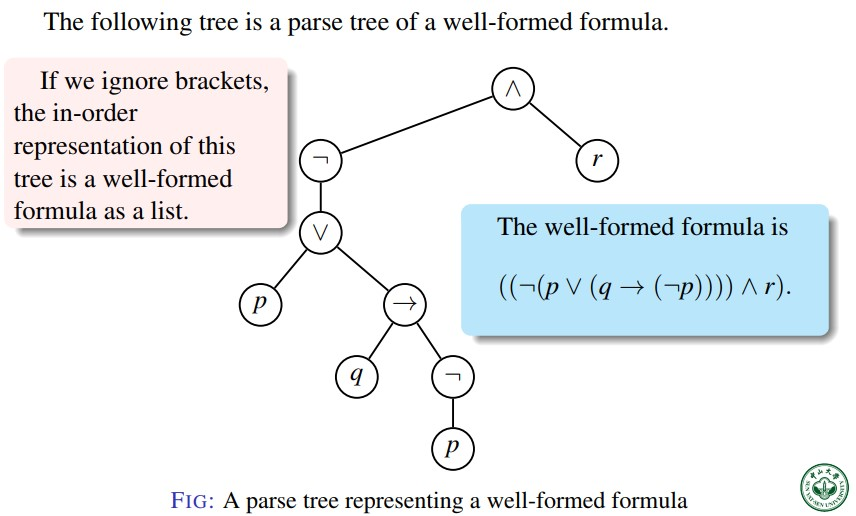
\includegraphics[width=0.8\linewidth]{fig/well-formed_formula.jpg}
\end{figure}

\subsection{语义}
\begin{definition}[模型(model)]
在前提$\phi_1,\phi_2,\ldots,\phi_n$和结论$\psi$上定义另一关系,记作
\[\phi_1,\phi_2,\ldots,\phi_n\models\psi\]
真值包括两个元素$T$和$F$,公式$\phi$的模型(model)或估值(valuation)是指对$\phi$中的每一原子命题都有一个真值指派(assignment)。
对$\phi_1,\phi_2,\ldots,\phi_n$的真值指派决定了$\psi$的真值,称为$\psi$的解释(interpretation),可表示为真值表中的一行。

如果对于所有$\phi_1,\phi_2,\ldots,\phi_n$的估值都为$T$,$\psi$也估值为$T$,那么称
\[\phi_1,\phi_2,\ldots,\phi_n\models\psi\]
成立(hold),且称$\models$为语义包含(semantic entailment)关系。
\end{definition}
\begin{theorem}[正确性(soundness)]
令$\phi_1,\phi_2,\ldots,\phi_n$和$\psi$都是命题逻辑公式,若$\phi_1,\phi_2,\ldots,\phi_n\vdash\psi$是合法的\footnote{假设$\phi_1,\ldots,\phi_n$为真,可以推出$\psi$为真},那么$\phi_1,\phi_2,\ldots,\phi_n\models\psi$成立。(事实上这两者是等价关系)
\end{theorem}

\begin{definition}[恒真式(tautology)/矛盾式(contradiction)]
命题逻辑$\phi$被称为恒真式当且仅当它在所有估值下都取值为$T$,也即$\models\phi$。
若在某个估值/解释$I_0$下值为$T$,则称其可满足。
若所有估值均为$F$,则为矛盾式。
\end{definition}
\begin{theorem}
若$\models\eta$成立,则$\vdash\eta$是合法的。
换句话说,若$\eta$是永真式,则$\eta$是定理。
\end{theorem}

\subsection{规范形式}
\begin{definition}[语义等价]
$\phi$和$\psi$都是命题逻辑的公式,称其等价当且仅当$\phi\models\psi$和$\psi\models\phi$成立,记作$\phi\equiv\psi$,也等价于$\models(\phi\to\psi)\land(\psi\to\phi)$成立。
\end{definition}
\begin{definition}[合取范式(conjunction normal form, CNF)]
BNF定义如下:
\begin{itemize}
	\item 文字(literal):$L::=p\mid\lnot p$
	\item 句子(clause):$D::=L\mid L\lor D$
	\item 公式(formula):$C::=D\mid(D)\mid D\land C$
\end{itemize}
例子如
\[(p \lor r) \land (\lnot p \lor r) \land (p \lor \lnot r)\]
\end{definition}

\begin{definition}[霍尔公式(Horn formula)]
若命题逻辑公式$\phi$能用下面的语法,表示成$H$的一个示例
\[P::=\bot\mid\top\mid p\qquad
A::=P\mid P\land A
C::=A\to P
H::=C\mid C\land H\]
则称$C$的每个实例为霍尔从句(clause)。
\end{definition}

\subsection{SAT求解器}
线性求解器只接受以下几种形式的公式
\[\phi::=p\mid(\lnot\phi)\mid(\phi\land\phi)\]
\begin{example}
$\phi=p\land\lnot(q\lor\lnot p)$,计算$T(\phi)=p\land\lnot\lnot(\lnot q\land\lnot\lnot p)$,则有语法树和DAG如下
\begin{figure}[H]
\centering
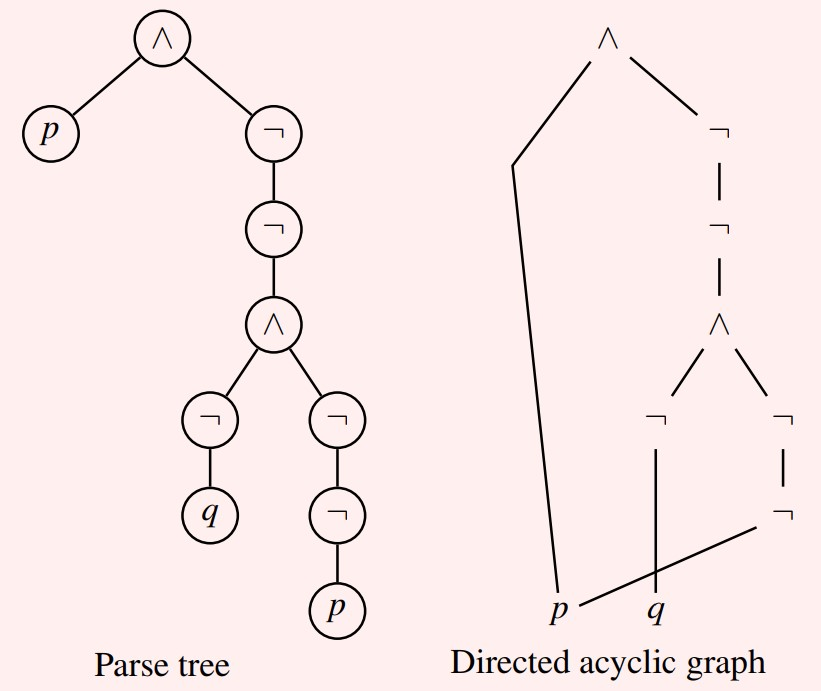
\includegraphics[width=0.6\linewidth]{fig/parse_tree_dag_eg.jpg}
\end{figure}
\end{example}